\documentclass[conference]{IEEEtran}

\ifCLASSINFOpdf
   \usepackage[pdftex]{graphicx}
\else
  \usepackage[dvips]{graphicx}
\fi

\usepackage{cite}
\usepackage{url}
\usepackage{booktabs}
\usepackage[justification=centering]{caption}
\usepackage{pifont}
\usepackage[para]{threeparttable}
% url.sty was written by Donald Arseneau. It provides better support for
% handling and breaking URLs. url.sty is already installed on most LaTeX
% systems. The latest version can be obtained at:
% http://www.ctan.org/tex-archive/macros/latex/contrib/misc/
% Read the url.sty source comments for usage information. Basically,
% \url{my_url_here}.

% correct bad hyphenation here
\hyphenation{op-tical net-works semi-conduc-tor}

\begin{document}
\bibliographystyle{IEEEtran}
% can use linebreaks \\ within to get better formatting as desired
\title{Enriching the Architecture Knowledge with Technology Design Decisions}


% author names and affiliations
% use a multiple column layout for up to three different
% affiliations
%\author{\IEEEauthorblockN{Michael Shell}
%\IEEEauthorblockA{School of Electrical and\\Computer Engineering\\
%Georgia Institute of Technology\\
%Atlanta, Georgia 30332--0250\\
%Email: http://www.michaelshell.org/contact.html}
%\and
%\IEEEauthorblockN{Homer Simpson}
%\IEEEauthorblockA{Twentieth Century Fox\\
%Springfield, USA\\
%Email: homer@thesimpsons.com}
%\and
%\IEEEauthorblockN{James Kirk\\ and Montgomery Scott}
%\IEEEauthorblockA{Starfleet Academy\\
%San Francisco, California 96678-2391\\
%Telephone: (800) 555--1212\\
%Fax: (888) 555--1212}}

% for over three affiliations, or if they all won't fit within the width
% of the page, use this alternative format:
%
\author{\IEEEauthorblockN{
Mohamed Soliman\IEEEauthorrefmark{1},
Matthias Riebisch\IEEEauthorrefmark{1} and
Uwe Zdun\IEEEauthorrefmark{2}}
\IEEEauthorblockA{\IEEEauthorrefmark{1}Department of Informatics,
University of Hamburg,
Hamburg, Germany\\
http://swk-www.informatik.uni-hamburg.de}
\IEEEauthorblockA{\IEEEauthorrefmark{2}Faculty of Computer Science,
University of Vienna, Vienna, Austria\\
Email: uwe.zdun@univie.ac.at}}

\maketitle

\begin{abstract}
%\boldmath
Decision-making is the core of the software architecture design. 
However, in order for the architect to take the right decisions, 
assistance is required for managing the complexity of the evolving
architectural knowledge, which encompasses the various types of architectural
solution, and design problems. In the past two decades, technology production
has increased significantly. Existing architecture knowledge approaches
support technology decisions by representing relations between
the different technology solutions, as well as problems. However, they do not
provide guidance for differentiating the candidate technologies according to
their offered qualities and drawbacks. Our main goal in this exploratory study
is to understand, how technology solutions are being considered by the
architects during the design process, and how can we enhance the existing
architecture knowledge concepts, in order to support the technology decision
making. Our contribution in this paper is a multi-viewpoint extension for
existing architecture knowledge models, which characterize the technology design
decisions, their reasoning and consequences. We verified our results through
practical real examples from architects and technologists. In addition, we
conducted interviews with experts to validate our proposed concept.
\end{abstract}

\section{Introduction}
Taking the right design decisions for crucial design issues is within the core
of software architecture. These decisions are distinguished by their
associated risks, which originate from the various unknowns that surround the
decision maker during the design process. The reason for such ambiguity is due
to the amount and diversity of the architectural solutions, and their different
capabilities to satisfy the system \textit{Architecture Significant Requirements
(ASRs)} \cite{BabarASR2013}, such that it's arduous to select accurately the
appropriate solutions for the different problems.

In order to assist the architect in exploring the design space, and
selecting the right combination of architectural solutions, approaches have been
proposed to model and manage the architecture knowledge. These approaches are
based on modeling the possible \textit{Architectural Design Decisions (ADDs)}
\cite{Jansen2005}. Design issues, architectural solutions, and the evaluations
for their different combinations are the main building blocks of this
architecture knowledge, which is characterized by its continuous evolution.

Architectural solutions can be classified into \textit{Conceptual Solutions} and
\textit{Technology Solutions}. The former are reusable abstract solution's
notions for design problems, which can be implemented differently in different contexts. This type include
patterns (e.g. architectural patterns \cite{Buschmann1996} and design patterns
\cite{Gamma1994}), as well as design tactics\cite{BassBook2012}.
On the other hand, technology solutions are concrete implementation solutions, 
which assist the architect to develop and realize the system, this include
frameworks, programming languages, standards and libraries. 
Both types of solutions are interrelated. In addition, both types impact the system 
functionality and quality differently.

The past two decades have seen a notable advancement in the reusability of
software components. This improvement supported the rapid development of
products and technologies with different capabilities in a short time, such that
the development productivity has increased exponentially, and
consequently, an increase in the technology vendors production, as well as the
open source community \cite{Boehm2006}. As a result, the
selection of the right technology product turn out gradually to be convoluted.

A recent survey \cite{Weinreich2013} on the types of architectural design
decisions and their documentation shows that around 25\% of a system decisions
are executive decisions, and most of them are technology decisions. Moreover,
technology decisions as well as structural decisions have been observed as the
mostly documented design decisions among other categories of decisions. The
survey participants indicated that technology decisions are taken early in the
design process, and it's quit hard to change them during the system
implementation. These results indicate and affirm the importance of technology
decisions for the software architect.

Even with their well known significance, the current methods for software 
architecture design (e.g. Attribute Driven Design \cite{Bass2003} and 
\cite{Bosch2000}), as well as pattern languages (e.g.
\cite{Avgeriou2005}) don't support the architect to make a choise among
different technology solutions. Alternatively, they focus on selecting a
combination of conceptual solutions as first class concepts for solving the
different design issues, presupposing a direct mapping from the conceptual
solutions to the technology solutions \cite{Kazman2013}.

Our main goal in this paper is to support the architect taking the technology
design decisions, through answering the following research questions:
\begin{enumerate}
\item \textit{RQ1: How does the architect conceive software technologies as
architectural solutions during the decision making process?}
\item \textit{RQ2: How can we model and relate technology decisions with
existing architecture knowledge elements?}
\end{enumerate}
In order to answer these questions, we conducted an explorative research
study. We started with a qualitative content analysis research process, followed
by refinement and validation interviews. The main contributions in this paper is
defining technology solutions as a set of architecturally significant aspects,
and proposing a multi-viewpoint extension for existing architecture
knowledge models to support the architect handling the technology decisions
during different design circumstances.

The rest of the paper is structured as follows. In Section \ref{sec:process}, we
describe and explain in details our research process. In Section
\ref{sec:aspects}, the idea of technology aspects is defined, followed by
Section \ref{sec:AK}, where the proposed architecture knowledge model for
technology decisions is proposed. In Section \ref{sec:results}, our validation
results for the interviews data anaylsis is presented, as well as a discussion
about the threads of validity for our study, and the related
work in the current state of the art is presented in Section \ref{sec:related}.
Finally, Section \ref{sec:conclusion} provides our conclusions and future work.
%%%%%%%%%%%%%%%%%%%%%%%%%%%%%%%%%%%%%%%%%%%%%%%%%%%%%%%%%%%%%%%%%%%%%%%%%%%%%%%%%%%%%%%%%%%%%%%%%%%%%%%%%%%%%%%%%%%%%%%
%%%%%%%%%%%%%%%%%%%%%%%%%%%%%%%%%%%%%%%%%%%%%%%%%%%%%%%%%%%%%%%%%%%%%%%%%%%%%%%%%%%%%%%%%%%%%%%%%%%%%%%%%%%%%%%%%%%%%%%
%%%%%%%%%%%%%%%%%%%%%%%%%%%%%%%%%%%%%%%%%%%%%%%%%%%%%%%%%%%%%%%%%%%%%%%%%%%%%%%%%%%%%%%%%%%%%%%%%%%%%%%%%%%%%%%%%%%%%%%
%%%%%%%%%%%%%%%%%%%%%%%%%%%%%%%%%%%%%%%%%%%%%%%%%%%%%%%%%%%%%%%%%%%%%%%%%%%%%%%%%%%%%%%%%%%%%%%%%%%%%%%%%%%%%%%%%%%%%%%
\section{Research Process}
\label{sec:process}
\begin{figure}
	\centering
		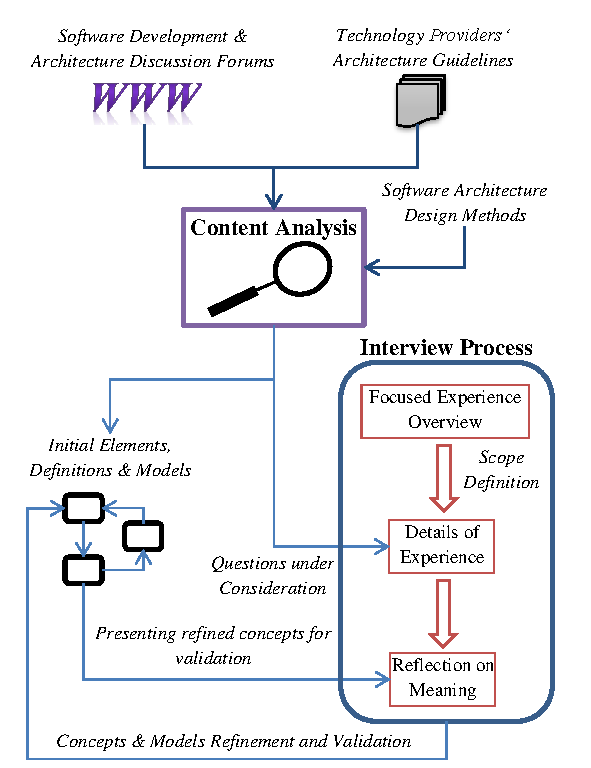
\includegraphics[scale=0.8]{ResearchProcessDiagram.pdf}
	\caption{Research Process Diagram.}
	\label{fig:ResearchProcess}
\end{figure}
In order to answer our research questions, we followed the research process as
shown in Fig. \ref{fig:ResearchProcess}. We divided our research process into
two main phases:
\begin{enumerate}
\item \textit{Data Gathering and Hypothesis Definition}: In this phase, our main
goal was to collect information about the technology decisions. We wanted to understand,
what are the primary factors, which make an architect choose or reject a certain
technology solution, and what are the scenarios he face during a technology
decision. In order to achieve this goal, we followed a qualitative content
analysis research method among different technology resources. As a result of
this phase, we formulated our initial hypothesis for the technology
decision concepts and models.
\item \textit{Hypothesis Refinement and Validation}: In order to refine and
validate our proposed concepts and models. It was important to align our
understanding with what architects in practice do in their work. Since
interview research method is the best method in discovering the human
experience \cite{seidman2006interviewing}. We conducted a set of
interviews with architects and experts, who are used to take technology
decisions frequently. This process helped us to improve our model, as well as to
validate our ideas.
\end{enumerate}
In the following sections, we explain both the content analysis and the
interview research processes respectively.
\subsection{Content Analysis}
\label{sec:contentanalysis}
Performing content analysis through technology
guidelines and social media technical web sites (e.g. Stackoverflow). This step result in our initial
concepts and models.

- Speak about the data, technology books and web sites, stack overflow.
	- The criteria for selection.
	- How are they prepared.
	- Initial Analysis
	
- Speak about the process of analysis
	- Classification. (Grounded Theory practicies)
	- Relationship between them.

- The role of litreture analysis in getting the concerns.

- Write in the content analysis, that it supported us to build an initial
hypothesis, and models.
\subsection{Interviews}
\label{sec:interviews}
As we were seeking experience in technology architectural decisions, several
factors have been considered in choosing the interview participants: 1) Their
experience in using and choosing technologies. 2) Their architecture
knowledge and design skills. 3) The size of the companies and systems, they are
working in or have worked in before. 4) Their interest and motivation to
participate in the study. Before choosing the interviewed experts, we identified
more than 20 candidate experts through our personal connections. We evaluated
them based on the mentioned criteria, to settle on the 6 participated experts.
It's interesting to mention that, even though some of the candidate experts work
in the role of a software architect in their companies. However, they don't take
technology decisions! In these companies, the architecture decisions are divided
between two different roles, the software architect, who design the system
conceptually, and the technology consultant who choose the technologies.
Therefore, we included in our study experts, who only take technology decisions. 

The interviewed experts work, or worked before in software houses or IT service
companies, with more than 100,000 employees. All the experts have either a
Bachelor or Master degree in computer science or engineering. Due to the fact
that the participants live and work in different cities, the interviews have
been conducted remotely through telecommunication softwares, which facilitated
the interviews recording.

We followed a 3 phase interview process as proposed by Seidman
\cite{seidman2006interviewing}:
\begin{table}[t]
\centering
\caption{Interview Participants Experience Overview}
\begin{tabular}{|c|c|c|c|c|}
\hline
\textbf{ID} & \textbf{\begin{tabular}[c]{@{}c@{}}Exp.\\ (Years)\end{tabular}} & \textbf{\begin{tabular}[c]{@{}c@{}}Technology \\ Background\end{tabular}}  & \textbf{Role}                                                    & \textbf{Industries}                                                                                                         \\ \hline
1           & 10                                                              & \begin{tabular}[c]{@{}c@{}}C/C++, \\ Microsoft Products\end{tabular}       & \begin{tabular}[c]{@{}c@{}}Technology \\ Consultant\end{tabular} & \begin{tabular}[c]{@{}c@{}}NLP, Performance \\ Critical Systems, \\ E-Commerce\end{tabular}                                 \\
2           & 13                                                              & \begin{tabular}[c]{@{}c@{}}Microsoft \\ Technologies\end{tabular}          & Architect                                                        & \begin{tabular}[c]{@{}c@{}}Flight, \\ Communications, \\ Social Media, \\ Reservation,\\ Retail and Education.\end{tabular} \\
3           & 11                                                              & Java / J2EE                                                                & \begin{tabular}[c]{@{}c@{}}Technology \\ Consultant\end{tabular} & \begin{tabular}[c]{@{}c@{}}Billing, \\ Medical-care, \\ E-commerce\end{tabular}                                             \\
4           & 9                                                               & Java / J2EE                                                                & \begin{tabular}[c]{@{}c@{}}Enterprise \\ Architect\end{tabular}  & \begin{tabular}[c]{@{}c@{}}Telecom, \\ Costing \& Billing, \\ Oil \& Mining,\\ Military\end{tabular}                        \\
5           & 10                                                              & \begin{tabular}[c]{@{}c@{}}Java / Integration \\ Technologies\end{tabular} & \begin{tabular}[c]{@{}c@{}}Technology \\ Consultant\end{tabular} & \begin{tabular}[c]{@{}c@{}}Communications, \\ Transportation\end{tabular}                                                   \\
6           & 7                                                      
& Java / J2EE &
\begin{tabular}[c]{@{}c@{}}Technology \\ Consultant\end{tabular} &
\begin{tabular}[c]{@{}c@{}}E-Government, \\ Automotive\end{tabular}                 
\\ \hline
\end{tabular}
\label{tab:Interviewparticipants}
\end{table}
\begin{enumerate}
\item \textit{Focused Experience Overview}: In this phase, we asked the
interviewees to answer several questions to show their experience in software
architecture, as well as their technology experience, projects and domain of
work. We made this step one or two days before the first meeting, which
supported us preparing the suitable questions which align with the participant's
context and experience. Table \ref{tab:Interviewparticipants} shows a brief
for the experience overview of the participants.
\item \textit{Details of Experience}: In this phase, we intend to learn from the
participant's experience, in order to refine and validate our concepts. Our
initial hypothesis, that we concluded from the content analysis phase helped us
to direct our questions and discussion. In order to do this, we mapped each
concept in the hypothesis with one or more interview questions, which has been
customized based on the result from the first phase. During the interview, we
were giving the space for the interviewees to explain and express their opinion,
and tell us about their experiences, which was the main feedback in this meeting
to verify and improve our concepts. The result from this meeting is a set of
real practical examples from each participant's experience, which either align,
or improve or contradict with our initial hypothesis. In the following sections,
we are going to state some of the \textit{Interview Questions (IQ)} that we asked to the
experts, as well as their responses and examples.
\item \textit{Reflection on the Meaning}: After the first meeting, we were able
to refine and verify our initial concepts, through the examples and discussions
presented by the participants. However, it was important to validate our
interpretation between the experience examples and the proposed
concepts. Therefore, in the second meeting, we focused on discussing the
proposed hypothesis concepts, and relating it to the mentioned experiences.
First, we explained our research goal, and the initial concepts and models, and
for each concept, supported with an example from the participant's experience, we asked
the interviewee, if this concept align with their understanding and practice.
Based on their feedback, we either validate or change or reject a certain
concept. Section \ref{sec:results} presented our evaluation results for the
proposed concepts, based on the interviewee feedback.
\end{enumerate}
For both interviews and for each participant, we recorded and transcripted the
interviews, to allow us analyzing the discussion. The length for each interview
was between 60 and 120 minutes. The difference in duration between the first and
the second interview for each participant is between 2 and 7 days.
\section{Architecturally Significant Technology Aspects}
\label{sec:aspects}
Technology solutions can be classified into two main categories
\cite{Zimmermann2009}\footnote{O. Zimmermann et. al named the descriptive and
executive solutions, as technologies and products respectively.}:
\begin{enumerate}
\item \textit{Descriptive Technology Solutions}: They are detailed
specifications, which describe the implementation of a certain solution. This
include languages, such as programming languages, as well as standards such as
protocols (e.g. Http) and encoding formats (e.g. XML).
\item \textit{Executive Technology Solutions}:
They are binary solutions, which support the development and implementation of
the system solution. This include frameworks, libraries and development
tools.
\end{enumerate}
Each of these technology solutions embodies different aspects, which are
designed and implemented within the technology. These aspects combine many
details about the technology solution. Consequently, it was interesting for us
to ask the participants, ''\textit{IQ: Should the architect know all the
technology details, in order to take the right ADDs? and, which technology solution's aspects should
she know about?}'' L. Bass et. al \cite{BassBook2012} listed
several important considerations in choosing a technology solution, such as the capabilities of
the development tools, the intimacy of the development community with this
technology, the possible external support, the drawbacks of the technology, and
the compatability of this technology with the existing technology stack.

One of the interview participants mentioned that \textit{''The architect
doesn't need to know the technology in depth. However, he need to know the
differences between the different technologies, their benefits and drawbacks,
regarding performance, company support, \ldots''}, another answered \textit{''He
need to know how technologies work from a high level, considering its learning curve,
the development effort, usability, \ldots''}.

Based on our analysis and the interview's discussions, we define in this section
the different types of \textit{Architecturally Significant Technology Aspects
(ASTAs)}. They are the principal and distinctive technology solution's
charachteristics, which distinguish the technology solution from other
alternative solutions, and consequently support or influence the architectural
design decision. In other words, these aspects qualify such a technology
solution to be selected by the architect to satisfy one or more ASRs. Moreover,
they act as considerable ramifications for an executive technology decision.

ASTAs can be viewed as either \textit{Features} or \textit{Limitations}. The
features are the merits, which the technology solution provide. Each feature
provide certain capabilities, which impact one or more of the architectural
concerns. On the other hand, limitations are either technology features, which
are missing in this technology solution, even though they exist in other
alternative solutions, or they are well-known existing features’ drawbacks,
which need to be considered by the architect during the decision making. Both
features and limitations act as different sides of the same coin, such that a
feature offered by a technology can be seen in a certain context as an
excellence, while in another, it can be seen as a hurdle.

One of the interview participants mentioned \textit{''Even though Java provide
an important feature for code portability among different platforms, this is a
significant drawback for our development, which seek native components
development. This makes us always favor C as our development technology.
Neverthless, it lacks such a platform independent feature''}.

ASTAs can be classified with respect to the capabilities provided by the
technology solution to the architect into different types. In the following
paragraph, we list and define the types of ASTAs. The definition is clarified
with examples from our analysis and interview practical experiences. In
addition, table \ref{tab:astasandconcerns} shows the relationship between each
aspect type and the different architectural concerns \cite{LagoConcerns}.
\begin{table}[t]
\centering
\caption{The relationship between ASTAs and Architectural Concerns}
\label{my-label}
\begin{tabular}{|c|c|}
\hline
\textbf{ASTA Type}                                             & \textbf{Influenced Architectural Concerns}                                                                             \\ \hline
\begin{tabular}[c]{@{}c@{}}Development \\ Aspect\end{tabular}  & \begin{tabular}[c]{@{}c@{}}Development Time, Training Time, \\ Maintainability, Testability, Evolvability\end{tabular} \\
\begin{tabular}[c]{@{}c@{}}Configuration\\ Aspect\end{tabular} & Training Time, Maintainability, Configurability                                                                        \\
\begin{tabular}[c]{@{}c@{}}Runtime \\ Aspect\end{tabular}      & \begin{tabular}[c]{@{}c@{}}Performance, Reliability, Security, \\ Accuracy, Portability, Reusability\end{tabular}      \\
\begin{tabular}[c]{@{}c@{}}Operational\\ Aspect\end{tabular}   & Manageability,  Supportability, Availability                                                                           \\
\begin{tabular}[c]{@{}c@{}}Integration \\ Aspect\end{tabular}  & Interoperability, Inter-process communication                                                                          \\
HCI Aspect                                                     & Usability                                                                                                              \\
Business Aspects                                               & \begin{tabular}[c]{@{}c@{}}Cost of Ownership, Openness, \\ Development Time, Training Time\end{tabular}                \\
Storage Aspect                                                 & Data Accessability                                                                                                     \\ \hline
\end{tabular}
\label{tab:astasandconcerns}
\end{table}
\begin{enumerate}
\item \textit{Development Aspects}: They provide the ability to develop or
extend an implementation for a solution through a development environment, which
comprises programming languages, compilers, libraries and possibly development
tools. Each of the contained development environment’s solutions has
consequently their own ASTAs. Such an aspect could be the rationale for
the architect to choose this technology. For example, one of the interview
participants mentioned the following: \textit{''We prefered to use the Springer
MVC framework over other frameworks, because it's easier to develop. In addition,
it's supported with better documentation, which make it easier to learn''}
\item \textit{Configuration Aspects}: They provide the ability to
configure an existing implemented solution through data changes.
Each of these aspects is associated with a configuration method, with a certain
complexity of changing. This type of aspects has a similar impact on the
architectural concern as the development aspects. An example from our content
analysis is the Windows Communication Foundation (WCF) technology, which is
based on adjusting an XML configuration file to specify the required
communication mechanism. The complexity of such a configuration can impact the
development and deployment effort.
\item \textit{Runtime Aspects}: They provide either existing and compiled
software components, which implement solutions with a certain quality,
or a forecasted quality for a possible development at certain conditions. An
interview participant described an experience about a certain database
management system limitation \textit{''After 1 year, the amount of data in the
database reached more than 20 billion records. We discovered that the performance of
data processing operations is degrading exponentially with the increase in the
amount of data, this technology limitation derived us to take an architectural
decision to replace such a database management system''}
\item \textit{Human Computer Interface (HCI) Aspects}: They provide a user
visible functionality implementation. These aspects are concerned with the
usability quality attribute of the technology. In certain situations, the system
usability act as the main concern of the stakeholders, as mentioned by an
interviewee \textit{''What motivated our design options is the usability
features provided, at that point, we wanted to choose between HTML 5, Web 2.0 and
Microsoft Silverlight''}
\item \textit{Integration Aspects}: They provide the ability for the technology
to integrate with other technologies. Such an aspect is quit important to be
considered, speacially after the executive decisions, which act as constrains on
the design decisions. For example, It's important to know, How can we communicte with
the DB2 database on mainframe from windows server.
\item \textit{Storage Aspects}: They provide the ability for the technology to
store data, considering the data format, data size and the ability to access and
manipulate the data. For example, some technologies provide the ability to store
data in an XML format, which set constrains on the possible size of the data,
and provide features and limitations for data accessability and manipulation.
\item \textit{Operational Aspects}: They provide the ability for the technology
to monitor and manage the processing of the system during execution. An
important example for this aspect is the performance monitoring tools associated
with some technology solutions.
\item  \textit{Business Aspects}: They are concerned with the price, licenses,
and the company and community support for this technology solution.
\item \textit{Abstract Aspects}: These are aspects which are provided by this
technology. However, they are actually implemented by another technology
solution. They represent a relationship to other technology solutions, which the
technology is based on. For example, the IBM Portlet Factory is based on the web
processing of the IBM Websphere.
\end{enumerate}
\section{Architecture Knowledge for Technology Design Decision}
\label{sec:AK}
\begin{table}[t]
\centering
\caption{Architectural knowledge viewpoints and their associated concerns}
\label{my-label}
\begin{tabular}{|l|}
\hline
\multicolumn{1}{|c|}{\textit{\textbf{ASTAs Relationship Viewpoint}}}                                                                   \\ \hline
\begin{tabular}[c]{@{}l@{}}What are the features and limitations of a technology solution which can \\ impact the ADD?\end{tabular}    \\
\begin{tabular}[c]{@{}l@{}}What are the dependencies between the different technology solutions, which \\ impact the ADD?\end{tabular} \\ \hline
\multicolumn{1}{|c|}{\textit{\textbf{Technology Decision Making Viewpoint}}}                                                           \\ \hline
\begin{tabular}[c]{@{}l@{}}What are the possible technology solutions for a certain architectural \\ design problem?\end{tabular}      \\
\begin{tabular}[c]{@{}l@{}}What are the project factors which influence the selection of a \\ technology solution?\end{tabular}        \\
\begin{tabular}[c]{@{}l@{}}Which technology solution is better than the others to fulfill a \\ certain requirement?\end{tabular}       \\
What are the different sources for technology solutions evaluations?                                                                   \\
Which technology evaluation sources or methods are suitable for this problem?                                                          \\ \hline
\multicolumn{1}{|c|}{\textit{\textbf{Technology Decision Consequences Viewpoint}}}                                                     \\ \hline
What are the consequences of selecting a certain technology solution?                                                                  \\
What are the possible solutions for a technology limitation?                                                                           \\
What is the cost of overcoming a certain technology limitation?                                                                        \\ \hline
\end{tabular}
\label{tab:viewpoints}
\end{table}
The sequence and path of the design decisions depend on many different factors
and forces \cite{AvgeriouForces} which drive or obligate the
architect to go in this direction. Each project and domain can have a different
situation, and a different decision making path, which is different than the
others. As mentioned in Sec. \ref{sec:process}, part of our content analysis and
hypothesis formulation process is to analyze existing state of the art
approaches for taking technology decisions. 

Technology decisions in the current software architecture design approaches are
addressed differently depending on the domain, and the proposed approach. Based
on our analysis, technology decisions can be classified into two main types:
\begin{enumerate}
\item \textit{Executive technology decisions}: They are decisions, which are
usually not taken by the architect. However, they are being taken due to business or
social factors. For example, an approach \cite{Ariyachandra2010200} analysed the
different management factors for choosing a data warehouse system. Technology
decision are sometimes being considered as constrains by architectural
design methods. For example, H. Gomaa et. al \cite{Gomaa1996} proposed an
architecture design process for distributed systems, where he considered the impact of technology constrains
on the system components structure. In other words, on the system conceptual solution.
\item \textit{Liberated technology decisions}: They are technology decisions
which can be selected based on the project ASRs, architectural concerns and
design factors, and the architect is usually responsible on taking them. In this
case, the architect need to choose a technology among different existing options
to realize his design \cite{BassBook2012}. For each solution domain, several
approaches are proposed to select between different technologies. For example,
\cite{BigDataMedvidovic} provide an elucidation for architecting data intensive
systems, considering the different design factors (e.g. Data volume and
dissamination), as well as the possible technology solutions, their benefits and
limitations. Similarly, comparisons between technologies (e.g.
\cite{ZimmermanWebServiceRest} and \cite{ZdunMiddelwareEv}) evaluate the
technologies' features and limitations, in order to support the architect
choosing between them.
\end{enumerate}

Based on these identified types from the current state of the art, as well as
the feedback from the interviewee, we identified several concerns, which are
important for the architect to handle the technology design decision. We grouped
the concerns into three main scenarios, ASTAs exploration, technology design
decision making and technology decision consequences. These scenarios align with
the different situations, that the architect can face during his decisions sequence.

In order to answer our second research question RQ2, we propose a model for the
architecture knowledge (AK) to support the architect in making the technology
decision. The model is based on the reusable design decision concept proposed by
O. Zimmermann \cite{Zimmermann2009}. In order to facilitate exploring and making
use of the knowledge during the decision making, we believe that the AK can be viewed from
multiple different viewpoints, such that each viewpoint supports one of the
previously mentioned three scenarios. Table \ref{tab:viewpoints} shows the list
of the drived concerns associated with their viewpoint. In the following
sub-sections, we outline each of these AK viewpoints, supported with examples.
\subsection{ASTAs Exploration Viewpoint}
\begin{figure}[b]
	\centering
		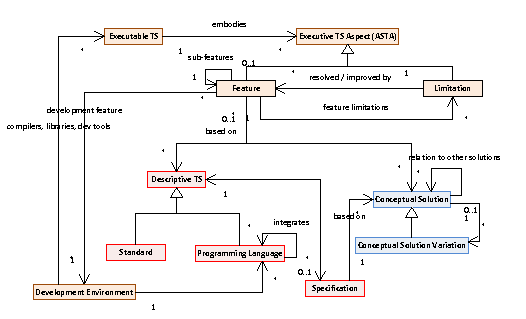
\includegraphics[scale=1.0]{SolutionsFeatuersRelationsModel.pdf}
	\caption{Modeling the relationships between the different architectural
	solutions and the different aspect types}
	\label{fig:SolutionAspectsRelations}
\end{figure}
Fig. \ref{fig:SolutionAspectsRelations} presents a meta-model to show the
relationship between the different types of aspects and the different software
architectural solutions, including conceptual, descriptive and executive
technology solutions. Each executive technology solution (e.g. Framework,
Product, \ldots) encapsulates a set of interrelated ASTAs, which decide the
influence of this technology solution on the architectural concerns.
Additionally, each of the ASTAs can be optionally based on a descriptive
technology solution (e.g. a standard or design specification) or on conceptual
architectural solution (e.g. an architectural pattern or tactic).
\begin{figure*}
	\centering
		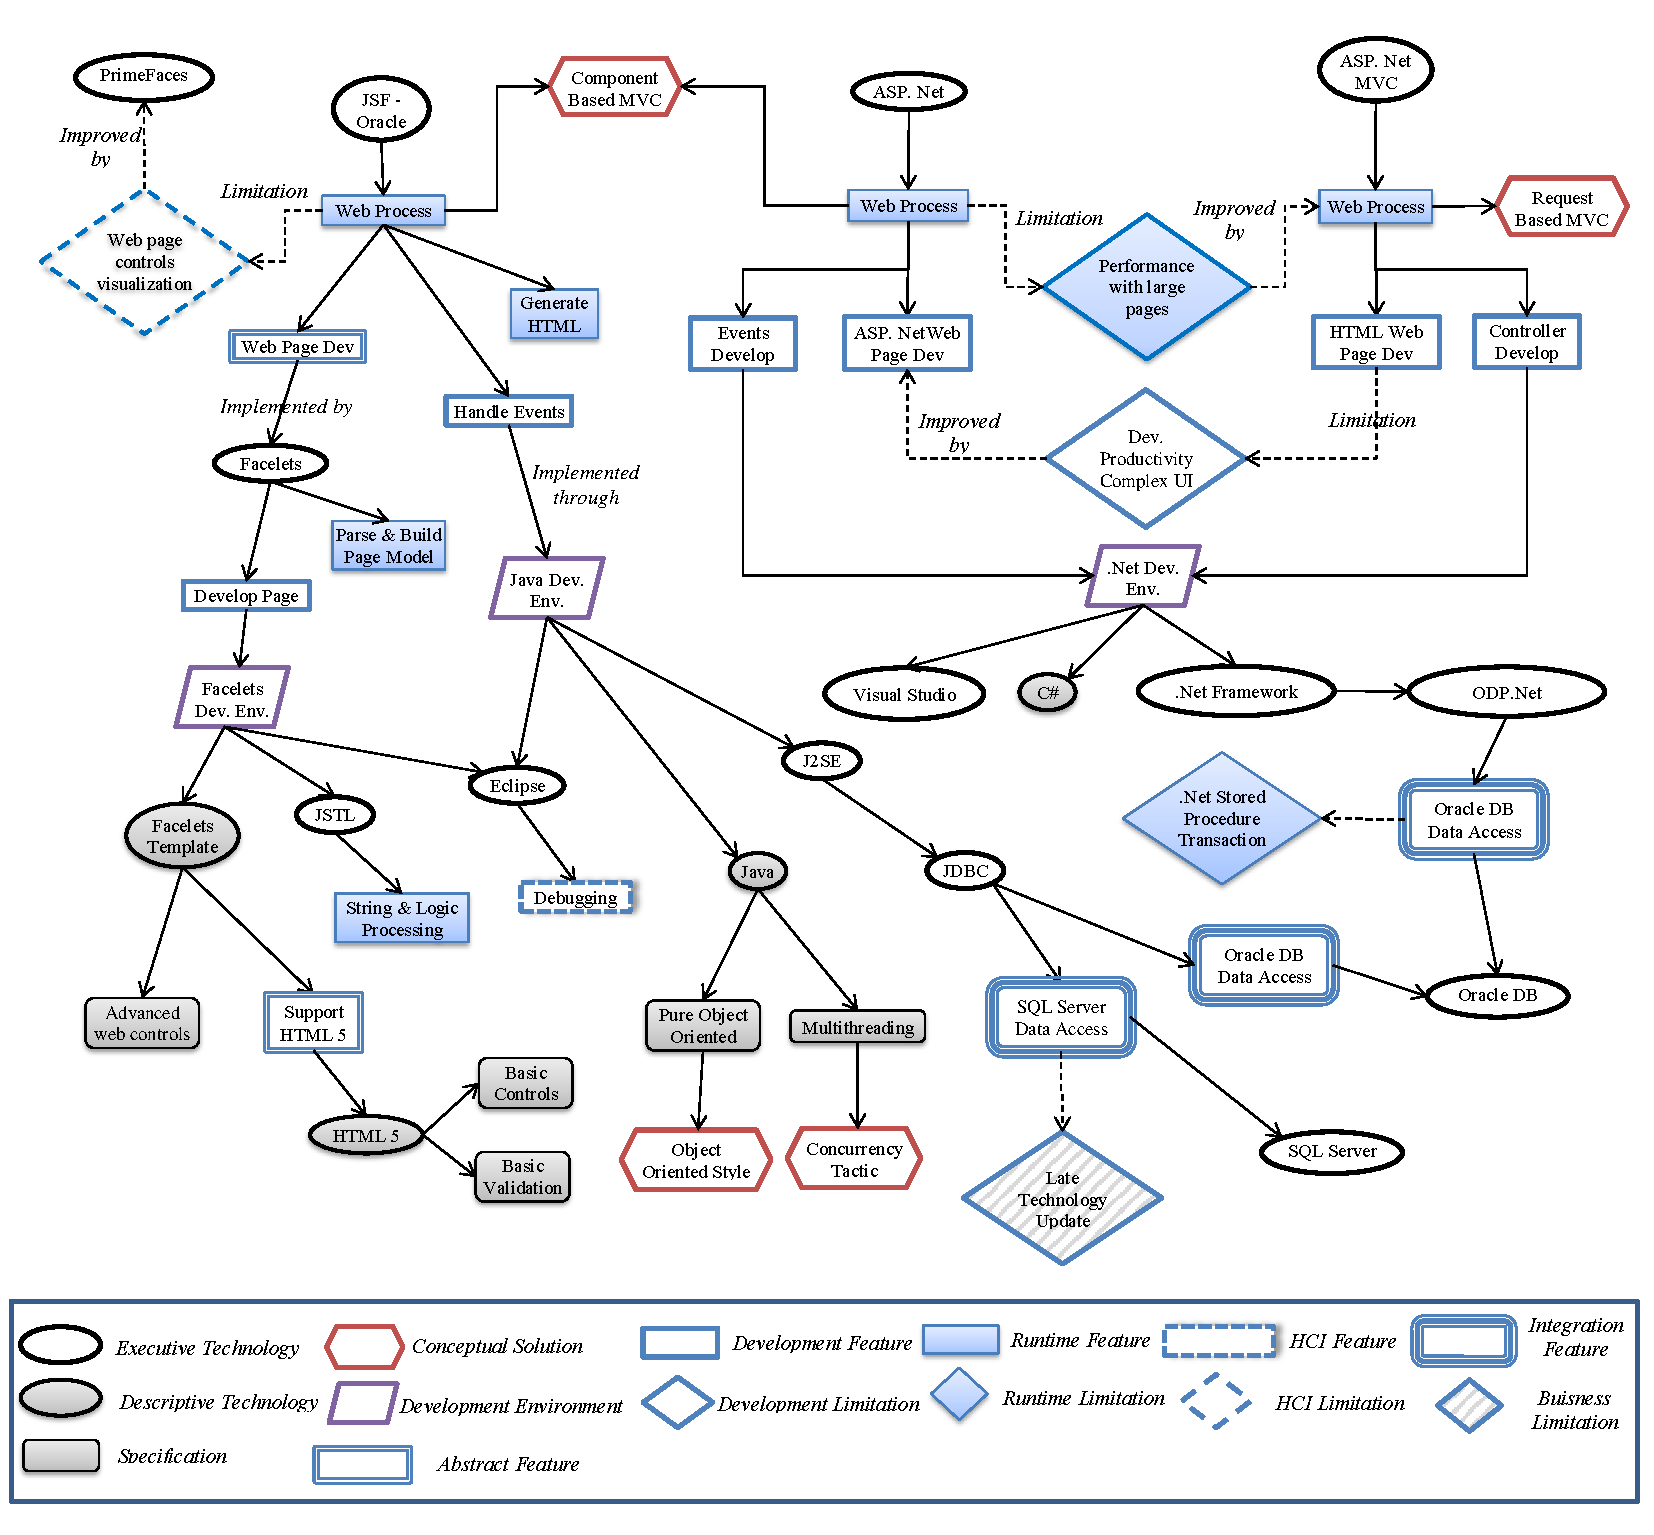
\includegraphics[scale=0.65]{TechnologyFeaturesExample.pdf}
	\caption{An example for modeling technology solutions' features.}
	\label{fig:TechnologyAspectsStructureExample}
\end{figure*}

Each technology solution encapsulates a tree of ASTAs, which include features
and limitations. These technology's ASTAs provide the relationship with the
architectural concerns, and connect the different technologies togethor. Fig.
\ref{fig:TechnologyAspectsStructureExample} shows an example for a partial
technologies' ASTAs knowledge base, which has been created through our content
analysis activity, integrated with the industrial examples mentioned by the
interviewed experts. For example, JSF is a web user interface technology, which
provide a component based web process \textit{'Runtime Feature'}, and based on
this feature, several sub-features are associated. This include developing the user
interface, which is actually based on another technology solution 'Facelets'.
Therefore, JSF provides an \textit{'Abstract Feature'}, which is actually
implemented by the Facelet framework. On the other hand, JSF provides a Java development
environment \textit{'Development Feature'} to handle events. This environment
incorporates development tools, and the Java programming
language with its pure object oriented style.

In addition, Fig. \ref{fig:TechnologyAspectsStructureExample} shows 3 web
interface technology solutions, JSF, ASP.Net and ASP.Net MVC. The three technologies are
based on the MVC architectural pattern. However, they are based on different
pattern variations. This difference in pattern variation triggers a difference
in their ASTAs. For example, the ASP.Net provide a feature for faster and easier
development environment than the ASP.Net MVC, which can be viewed as a
\textit{'Development Limitation'}. On the other hand, ASP.Net has a
\textit{'Performance Limitation'} in building web pages with rich user
interface, due to the fact, that Component-based MVC need to store the view
state of each UI control.

In addition, Fig. \ref{fig:TechnologyAspectsStructureExample} shows 2 examples
for the \textit{'Integration Feature'} between technologies. The .Net
development environment can communicate with Oracle databases through the ODP.Net library,
while the Java development environment can communicate with Microsoft SQL Server
through the JDBC SQL Server data access library. Both integration features are
associated with a \textit{'Runtime and Business Limiations} respectively. The
former  is due to a drawback in executing transactions, while the latter is a business
limitation, which is due to company support.
\subsection{Technology Decision Making Viewpoint}
\label{sec:Design}
Design reasoning is the logic that the architect use when developing an
architectural solution. Several theories have been proposed, which try to depict
how the architect think about a solution for a design problem. This include
deductive and inductive reasoning, as well as problem and solution driven design
strategies \cite{TangReasoningStrategy, TangBiasing}.

During our interviews, we asked all the participants the following question:
 \textit{IQ: What are the steps you take to choose between a list of possible
technology solutions?} It was not surprising that each participant described a
different reasoning process than the others. However, all participants shared a
commen set of elements, which they consider in selecting the technology
solution, even though, they are used in a different order. Therefore, the
"Technology Decision Making" AK viewpoint contains and relates the different
elements, which are necessary to assist the architect for taking a liberated
technology decision, such that it can align with the different design reasoning
methods.
\begin{figure}
	\centering
		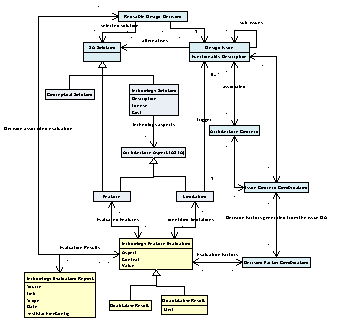
\includegraphics[scale=1.6]{TechnologyDecisionMakingView.pdf}
	\caption{A diagram showing an example for following the proposed reasoning
	process.}
	\label{fig:TechnologyDecisionMakingView}
\end{figure}
Fig. \ref{fig:TechnologyDecisionMakingView} shows the meta-model for the
"Technology Decision Making" viewpoint. At the core of the model are the design
issues, which are the architecture design problems facing the architect. Each
design issue is associated with a set of alternative architectural solutions. An
architectural solution can be either a conceptual solution, or a technology
solution, or even an embedded feature within a certain technology solution,
while a design issue can be triggered from an ASR, or a conceptual
solution \cite{Zimmermann2009,Soliman2014}, or a technology solution limitation.

Even though, each of the interview participants described different steps in
choosing a technology solution, we can still group their description into the
two main reasoning types identified earlier:
\begin{enumerate}
\item \textit{Deductive problem driven}: In this process, the architect starts
by analyzing the design issue, and its associated architectural concerns.
For example, in choosing between different middleware technologies,
interoperability, performance, security and development time should be
considered. For each of theses concerns, several factors are associated; the
technology at the client and server, the size and structure of the transfered
data, the network between the two sides, and the development team skills
respectively. Based on these factors, the architect can start evaluating the
different technology features. Two evaluation methods have been mentioned
by the interviewees to evaluate the technology features, the prototype and the
evaluation reports (e.g. benchmarks). Additionaly, the architect can estimate
the feature quality attribute based on the conceptual solution, which this feature
based on (e.g. evaluation for architectural patterns \cite{Bode2010}). By the
end of the process, the architect need to make trade-offs among the different
concerns \cite{BabarICSE2005}.
\item \textit{Inductive solution driven}: In this process, the architect starts
by checking other experiences which have similar situations. In other words,
design decisions which have been taken in different projects but at similar
circumstances, and based on matching both conditions, the architect choose the
suitable technology solution. We argue that the Executive technology
decisions cannot be reused in other projects within the context of software
design (maybe arguably reused in a business context), as their justification is
not architecture based. On the other hand, Liberated technology decision are
reusable, such that similar architectural concerns and factors could be repeated
among different projects.
\end{enumerate}
Even though, our main research goal is not to drive a design process. It is
important to understand, the different reasoning methods that the architect use,
in order to identify the important architecture knowledge elements and their
relationships.
\subsection{Technology Decision Consequences Viewpoint}
\label{sec:consequence}
Executive design decisions are decisions which are strongly influenced from the
business environment. In other words, the main motivation and reasons for taking
these decisions are business, financial, political or even social factors, and
they are usually not taken by the software architect, and act as constrains
on the other types of architectural design decisions \cite{Kruchten2006}.

During our interviews, we asked the participants about the factors which impact
the technology decisions. All of the participants mentioned the executive
decision motif, as one of the main types of the technology decisions.
Neverthless, each participant gave a different example for an executive
decision. For example, one of the participants mentioned \textit{''The sales
department was able to sell a certain technology product, which is developed by
the company. Thus, we were forced to use this technology, even though it's not
suitable to the customer requirements''}, another participant said \textit{''The
customer has an Oracle DB server licenses, while our vendor supports Microsoft products.
In this situation, we had to make a hybrid solution, which combine both
technologies to satisfy both sides!''}.

We believe that these types of decisions have a significant impact on the system
architecture, even though, they are not taken by the architect. Moreover, the
architect cannot change the fact, that these decisions are forced on the system
architecture. Hence, the architects try to understand their consequences and
ramifications, and to adapt and adjust the system on their constrains. In
addition, understanding the executive decision consequences can support the
architect to negotiate with the business partners, as a way to clarify the
possible costs and losses.

Either if an executive or liberated technology decision has been taken, it's
important for the architect to know the consequences of choosing a certain
technology solution. During the interviews, we asked the participants the
following question: \textit{IQ: What is important for an architect to do after
an executive technology decision have been taken?} Based on their answers, we
identified several decision consequences, which are modeled in the ''Technology
Decision Consequences'' AK viewpoint.
\begin{figure}
	\centering
		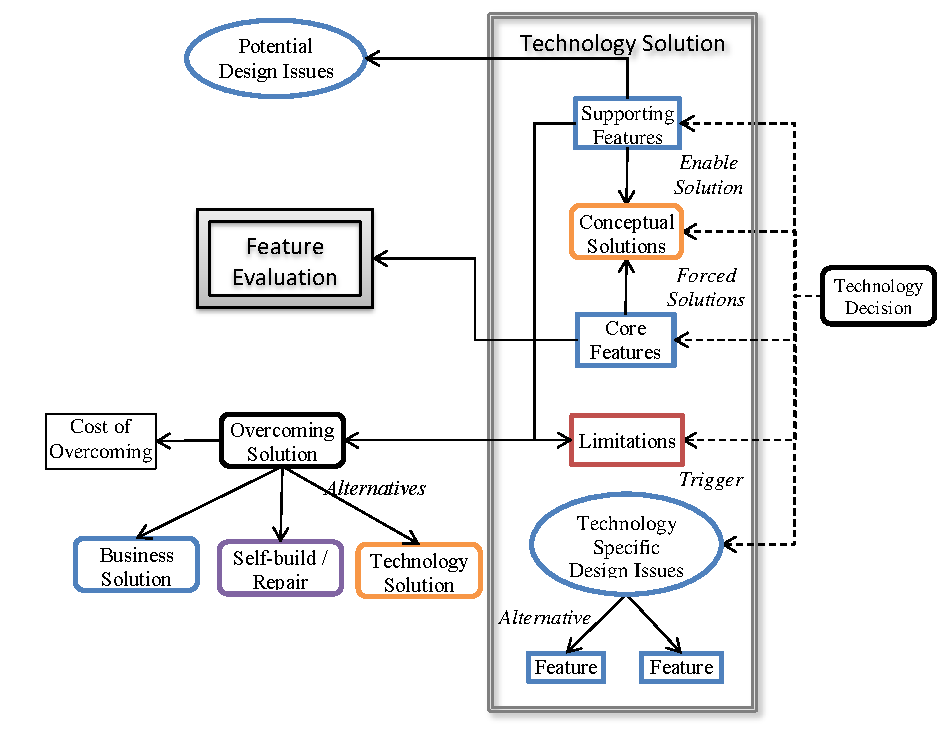
\includegraphics[scale=0.5]{TechnologyDecisionConsequences.pdf}
	\caption{A diagram showing a model which describes the different types of
	consequences of selecting a technology solution.}
	\label{fig:TechnologyDecisionConsequences}
\end{figure}
Fig. \ref{fig:TechnologyDecisionConsequences} shows a meta-model for the
viewpoint. We can divide the technology decision ramifications into the
following:
\begin{enumerate}
\item \textit{Forced Core Features Decisions}: Each technology solution has
principal features, which the solution is based on. Moreover, using these
features is mandatory to be able to use the technology solution for the system
implementation. For example, the technology deployment is a popular example for
the technology core feature. Relational database management systems core
features are the storage features for the tables structure. Sometimes core
features are based on a certain conceptual solutions, which force the architect
on designing the system based on the feature associated conceptual solution. For
example, the Spring framework features comprises a speacial variation and
constrains for the MVC pattern.
\item \textit{Enabled Supporting Features' Solutions}: Technologies also offer
supporting features which are not obligatory for the architect to use them. Even though, they can solve possible
potential design issues. For example, Microsoft Windows Communication
Foundation (WCF) framework offer different protocols (e.g. Http, TCP, FTP, \ldots)
for communication between different systems. The architect must not use all the
offered features directly. However, they can act as supporting features for
possible new requirements.
\item \textit{Limitation's Triggered Design Issues}: As we explained in the
previous sections, each technology solution comprises limitations, which
might influence the architectural concerns negatively. Each of the technology
limitations trigger an associated architectural issue, which need to be tackled
by the architect in order to overcome this drawback. During our interviews, all
of the interviewees mentioned the importance of handling these limitations as a
consequence for a technology decision. One of the participants mentioned
\textit{''It's not only important to know the technology limitations, but also the possible
solutions to overcome it, and the cost of each solution''}. For example, the JSF
framework has limitations, which impact the usability quality attribute.
Two main solutions were mentioned by the participant, using an additional
framework (e.g. Primefaces) to mend this problem, or hire a web designer to fix
the problem manually. Each solution has a different impact on the development
time and cost.
\item \textit{Technology Specific Design Issues}: Within the technology
solution, there can be possible different design options, which need to be
chosen by the architect. For example, a technology provide two ways of
deployment, a compatability and compliance mode.
\end{enumerate}
\section{Evaluation Results}
\label{sec:results}
\subsection{Interview Responses Analysis Results and Observations}
\begin{table}[t]
\centering
\caption{Interview Data Analysis Results\\\textit{++: Concept Contribution,
\ding{52}:
Concept Supported\\Y: Concept Accepted, N: Concept in Doubt}}
\begin{tabular}{|c|c|c|c|c|c|c|}
\hline
\textbf{Concept vs. Participant}                                                                                    & \textbf{1} & \textbf{2} & \textbf{3} & \textbf{4} & \textbf{5} & \textbf{6} \\ \hline
\textit{\begin{tabular}[c]{@{}c@{}}Technologies as Features \& Limitations\\
(Sec. \ref{sec:aspects})\end{tabular}}                   & Y          &
\ding{52} & \ding{52}  & \ding{52}  & \ding{52}  & \ding{52}  \\ \hline
\textit{\begin{tabular}[c]{@{}c@{}}Development \& Configuration Aspect \\ (Sec.
\ref{sec:aspects})\end{tabular}}                      & Y          & N         
& \ding{52}  & ++         & \ding{52}  & \ding{52}  \\\hline
\textit{Runtime Aspect (Sec. \ref{sec:aspects})}                                
& Y          & Y          & \ding{52}  & \ding{52}  & \ding{52}  & \ding{52} 
\\\hline
\textit{HCI Aspect (Sec. \ref{sec:aspects})}                                    
& Y          & Y          & Y          & \ding{52}  & Y          & \ding{52} 
\\\hline
\textit{Integration Aspect (Sec. \ref{sec:aspects})}                            
& Y          & ++         & Y          & Y          & ++         & --        
\\\hline
\textit{Storage Aspect (Sec. \ref{sec:aspects})}                                
& Y          & Y          & Y          & Y          & Y          & --        
\\\hline
\textit{Operational Aspect (Sec. \ref{sec:aspects})}                            
& Y          & --         & --         & --         & ++         & Y         
\\\hline
\textit{Business Aspect (Sec. \ref{sec:aspects})}                               
& Y          & Y          & ++         & Y          & Y          & --        
\\\hline
\textit{Decision Making Factors (Sec. \ref{sec:Design})}                       
& Y          & \ding{52}  & \ding{52}  & Y          & \ding{52}  & --        
\\\hline
\textit{Decision Making Concerns (Sec. \ref{sec:Design})}                       
& Y          & Y          & \ding{52}  & \ding{52}  & \ding{52}  & --        
\\\hline
\textit{\begin{tabular}[c]{@{}c@{}}Decision Making Evaluation \\ Report (Sec.
\ref{sec:Design})\end{tabular}}                       & Y          & --        
& --         & --         & --         & --         \\\hline
\textit{\begin{tabular}[c]{@{}c@{}}Decision Making Deductive \\ Problem Driven
(Sec. \ref{sec:Design})\end{tabular}}                & Y          & \ding{52}  &
\ding{52}  & \ding{52}  & Y          & Y          \\\hline
\textit{\begin{tabular}[c]{@{}c@{}}Decision Making Inductive \\ Solution Driven
(Sec. \ref{sec:Design})\end{tabular}}               & Y          & --         &
--         & --         & \ding{52}  & \ding{52}  \\\hline
\textit{\begin{tabular}[c]{@{}c@{}}Decision Consequences Core \& \\ Supporting
Features (Sec. \ref{sec:consequence})\end{tabular}}        & Y          & N         
& Y & \ding{52}  & Y          & --         \\\hline
\textit{\begin{tabular}[c]{@{}c@{}}Decision Consequences \\ Limitations (Sec.
\ref{sec:consequence})\end{tabular}}                       & Y          & Y     
& ++         & Y          & ++         & --         \\\hline
\textit{\begin{tabular}[c]{@{}c@{}}Decision Consequences Technology \\ Specific
Design Issues (Sec. \ref{sec:consequence})\end{tabular}} & Y          & Y          & Y          & Y          & Y          & --         \\ \hline
\end{tabular}
\label{tab:resultstable}
\end{table}
Table \ref{tab:resultstable} shows the data analysis results for the
interviewees' responses. In order to accuratly evaluate the feedback of the
participants for each of the explained concepts in the previous sections. We
designed several levels of responses:
\begin{enumerate}
\item \textit{Concept Contribution}: The participant mentioned based on
his experience a new concept or an improvement to a concept which was not
orignally part of the content analysis derived hypothesis.
\item \textit{Concept Supported}: The participant
supported the hypothesis concept with additional examples from his experience.
\item \textit{Concept Accepted}: The participant accepted
the proposed concept. However, she doesn't have an example from her experience
to support it.
\item \textit{Concept in Doubt}: The participant indicated that the concept is
unclear to her, or it does not align with her experience.
\end{enumerate}
The concepts which were charachterized as unclear by the majority of the
participants have been removed.

From the results, we can observe that most of the contributions of the
interviewed experts are in the technology solutions aspects (Sec.
\ref{sec:aspects}), while the least are in the decision making viewpoint (Sec.
\ref{sec:Design}). The reason for this is the nature of the concept. Most of
the participants mentioned that it's hard for them to articulate their decision
making process. Even with their experience examples, the explained processes
were not completely described. This makes it hard to contribute to this
viewpoint. In addition, we can observe that Limitation consequences (Sec.
\ref{sec:consequence}) and the Integration aspects (Sec. \ref{sec:aspects}) were
the mostly contributed concepts due to their importance to the participants.

Most of the concepts have been experienced by the participants during their
decision making experience, except two concepts: the storage aspect (Sec.
\ref{sec:aspects}), and the technology specific design issue within the
consequences viewpoint (Sec. \ref{sec:consequence}). The reason for the former
concept is the experience of the interviewed participants, which concentrates on
the solution architecture experience more than the data architecture, while the
latter concept was not obvious for the participants. In addition, few of the
contributed concepts have not been evaluated by all participants, due to the
fact, that the interviews have been conducted incrementally.
\subsection{Threads to Validity Assessment}
As all qualitative empirical studies, our study faces validity threats. This
section explain the construct, internal, and external validity threads, as well
as reliability of the study.
\subsubsection{Construct Validity}
In this type of validity, we are concerned with validating the accurate
representation of the initial content analysis hypothesis through the
interviews' questions, as well as the interviews' answers interpretation. In
order to map our initial hypothesis to the interview questions: First, we defined a set of
general questions, such that each question is related to a hypothesis concept
using a concept mapping. After our first phase of the interview process, we were
able to adapt these questions to align with the experts understanding, which
supported a more suitable explication of the hypothesis constructs. The
interviewee had no idea about our initial hypothesis during the second phase of
the interview process. In addition, the interview participants work in different
companies, and they don't know about each other. This prevented any interactions
between the different experts, as well as any possibility of hypothesis
guessing.

During the third phase of the interview, our main goal was to validate our
interpretation the experiences and examples mentioned during the second phase
of the interview. By presenting and explaining our concepts and relating it to
the examples mentioned by the participants, we were able to assure that we have
the right generalizability across the hypothesis constructs. In addition,
conducting the concept validation among all the participants supported us to
minimize biasing during the results interpretation. However, we based our
concept discovery and validation on 6 interviews, which is insufficient to cover
all the possible aspects of technology decisions. Therefore, we believe that
additional empirical studies are needed to extend the proposed concept (See Sec.
\ref{sec:conclusion}).
\subsubsection{Internal Validity}
In this type of validity, it's important for us to insure that the interview
setup supported us to drive the concluded results. In conducting our interview,
we followed a set of guidelines (e.g. \cite{InterviewGuide}) in questions
preparation, as well as in managing the conversation with the participant. With
each participant, we started with a general question, like ''IQ: What are the
factors which influence choosing a technology?'' during the participant answer,
we give the freedom for the expert to explain his answer, and we asked the
expert to focus on real experience examples. This supported us to interpret the
meaning. In some cases, we mentioned the same question twice, however, with
different ways to ensure that the participant provide the needed information,
without interrupting his speaking. In addition, the 3 phase process helped us to
have more than a chance to clarify our understanding to the examples or concepts
explained by the interviewees. Even though, it was originally assumed that all
experts should have the same level of experience, four of the interviewed
experts contributed to the concepts more than the other two. However, this ratio
shouldn't impact our results. Moreover, all experts supported us in the model
validation through the interview ''reflection of meaning'' phase.
\subsubsection{External Validity}
In this type of validity, we would like to insure that our interview study
supports us to generlize the concluded technology decision architecture
knowledge model among the different design situations. Regarding this aspect, we
have several threats of validation. We did not select the interview participants
randomely, as we depend on our network of experts. However, we made no control
on their mentioned experiences. As the different participants have experience in
different domains, we didn't focus our discussion on domain specific problems.
Even though, one of the participants have experience in embedded systems. The
interview focused on experiences and technologies used within information and
distributed systems domain. Moreover, we focused on the solution level of
software architecture during our discussion, more than the enterprise level.
\subsubsection{Reliability}
To support the reliability of measurement. We followed an intra-rater
reliability method, such that the 3rd phase of the interview insured that the
same concepts have been validated and evaluated by the 6 interviewed
participants, while the participants responses were recorded by a single
interviewer. All the interviews were conducted one-to-one with prepared
questions, which give the chance for each participant to give his opinion about
others inputs.
\section{Related Work}
\label{sec:related}
\subsection{Software Architecture Design Methods}
In the past two decades, several prominent software architecture design methods
(e.g. RUP 4+1 views, Siemens 4 views, CAFCR, Hoffmeister) have been suggested
and utilized in practice. The proposed methods target modeling the software architecture in
several views, such that each view comprises distinctive diagrams for modeling
the proposed solution, in order to satisfy the stakeholders' architectural
concerns. In addition, the methods provide several guidelines for the
correlation between the different viewpoints. Most of the methods dedicate a
viewpoint for the implementation or system realization. For example, one of the
RUP 4+1 views is the the development view, which model the proposed solution
technology components and connectors, providing guidelines for taking the
technology decisions, such as ease of development, software management and
reuse. However, the proposed architectural methods provide minimum support for a
concrete architectural knowledge base \cite{MethodsSurveyKruchten}.
Consequently, this makes the architects depend on their personal experience,
instead of reusing and learning from others experiences.
\subsection{Pattern Languages}
A pattern language is concerned with defining a group of patterns, which solve
related problems in the same domain. Moreover, some pattern languages provide
relationships between patterns, to support the architect taking the design
decisons through moving from one pattern to another. In the past two decades,
many pattern languages have been proposed (e.g. \cite{Buschmann1996}). However,
each pattern language address a different domain of problems. Typically, pattern
languages do not incorporate technology solutions as first class elements within
their network of decisions. However, each pattern provide optionally a list of
technology examples, which implement this pattern. A proposed pattern language
\cite{hezavehi2011pla} integrate technology solutions with pattern languages.
The proposed language model interrelationships between different technology
solutions, as well as an implementation relationship between technologies and
patterns. However, the suggested solution's network doesn't provide guidance for
decison making and reasoning.
\subsection{Software Architecture Design Decisions}
Since the paradigm shift \cite{Jansen2005} of perceiving the software
architecture as a set of architectural design decisions (ADDs), many approaches
have been proposed. Even though, all approaches are centered around the design
decisions notion, they tackle different problems. A recent survey
\cite{AvgeriouSurvey2014} on the architectural decisions field shows that most
of the approaches focus on modeling, documenting and capturing the ADDs rational
(e.g. \cite{Kruchten2006}, \cite{Heesch2012} and \cite{KruchtenEmperical2008})
for the sake of minimizing the software architecture erosion phenomena. However,
these approaches don't support the architect in reasoning about the design
decisons. Alternatively, other approaches (e.g. \cite{LagoMindset},
\cite{TangReasoning2008}) consider the design decision as a mean for reasoning
about the design problems. In other words, they try to model and
depict the different methods, that the architect can use to think about an
architecture design problem. Neverthless, they don't support a concrete reusable
architecture knwoledge.

A recent study on the software architecture knowledge
\cite{WeinreichSurvey} shows that, the current architecture knowledge approaches
have less support regarding architecture knowledge sharing and reuse.
Differentiating the reusable architecture knowledge from the project specific have been
considered by M. Ali Babar et. al \cite{BabarAK} and O. Zimmermann et. al
\cite{Zimmermann2009, Soliman2014}. The former approach considered a generic
knowledge component based solely on patterns, which can be selected during the design
decisions capturing. On the other hand, O. Zimmermann et. al proposed a reusable
architecture knowledge framework, with the design issues and architectural
solutions as the main elements, while the possible decisions' relations are
modelled between them. In addition, the decisions are divided based on their
granualarity into conceptual, technology and products. Even with the provided
support for modeling technology decisions, the approach proposed by O.
Zimmermann lacks the ability to distinguish between the different technologies'
capabilities from each other, such that it's hard for the architect to choose
the suitable technology solution for the project situation. We believe that the
approach proposed by O. Zimmermann is promising regarding architecture knowledge
reuse. Therefore, we based our approach based on his proposed model.
%%%%%%%%%%%%%%%%%%%%%%%%%%%%%%%%%%%%%%%%%%%%%%%%%%%%%%%%%%%%%%%%%%%%%%%%%%%%%%%%%%%%%%%%%%%%%%%%%%%%%%%%%%%%%%%%%%%%%%%
%%%%%%%%%%%%%%%%%%%%%%%%%%%%%%%%%%%%%%%%%%%%%%%%%%%%%%%%%%%%%%%%%%%%%%%%%%%%%%%%%%%%%%%%%%%%%%%%%%%%%%%%%%%%%%%%%%%%%%%
%%%%%%%%%%%%%%%%%%%%%%%%%%%%%%%%%%%%%%%%%%%%%%%%%%%%%%%%%%%%%%%%%%%%%%%%%%%%%%%%%%%%%%%%%%%%%%%%%%%%%%%%%%%%%%%%%%%%%%%
%%%%%%%%%%%%%%%%%%%%%%%%%%%%%%%%%%%%%%%%%%%%%%%%%%%%%%%%%%%%%%%%%%%%%%%%%%%%%%%%%%%%%%%%%%%%%%%%%%%%%%%%%%%%%%%%%%%%%%%
\section{Conclusion and Future Work}
\label{sec:conclusion}

\bibliography{literature_short}

\end{document}


